
\documentclass[12pt, a4paper, oneside, headinclude, footinclude]{article}

%----------------------------------------------------------------------------------------
%	REQUIRED PACKAGES
%----------------------------------------------------------------------------------------

\usepackage[
nochapters, 
beramono, 
eulermath,
pdfspacing, 
dottedtoc 
]{classicthesis} 

\usepackage{arsclassica} 
\usepackage{listings} 
\usepackage{minted} 
\usepackage[T1]{fontenc} 
\usepackage[utf8]{inputenc} 
\usepackage{graphicx} 
\graphicspath{{Figures/}} 
\usepackage{enumitem} 
\usepackage{lipsum} 
\usepackage{subfig} 
\usepackage{amsmath,amssymb,amsthm} 
\usepackage{varioref} 

%----------------------------------------------------------------------------------------
%	THEOREM STYLES
%---------------------------------------------------------------------------------------

\theoremstyle{definition} 
\newtheorem{definition}{Definition}

\theoremstyle{plain} 
\newtheorem{theorem}{Theorem}

\theoremstyle{remark} 

%----------------------------------------------------------------------------------------
%	HYPERLINKS
%---------------------------------------------------------------------------------------

\hypersetup{
colorlinks=true, breaklinks=true, bookmarks=true,bookmarksnumbered,
urlcolor=webbrown, linkcolor=RoyalBlue, citecolor=webgreen, 
pdftitle={}, 
pdfauthor={\textcopyright}, 
pdfsubject={}, 
pdfkeywords={}, 
pdfcreator={pdfLaTeX}, 
pdfproducer={LaTeX with hyperref and ClassicThesis} 
}


\title{\normalfont\spacedallcaps{DRAFT High Level Technical Design: World Bank Building Detection Proof of Concept}}

\author{\spacedlowsmallcaps{Krishna Bhogaonker}} 
 
\date{\today\\version 0.1}
\begin{document}

\renewcommand{\sectionmark}[1]{\markright{\spacedlowsmallcaps{#1}}} 
\lehead{\mbox{\llap{\small\thepage\kern1em\color{halfgray} \vline}\color{halfgray}\hspace{0.5em}\rightmark\hfil}} 

\pagestyle{scrheadings} 

%----------------------------------------------------------------------------------------
%	TABLE OF CONTENTS & LISTS OF FIGURES AND TABLES
%----------------------------------------------------------------------------------------

\maketitle 

\setcounter{tocdepth}{2}

\tableofcontents 

% \listoffigures 

% \listoftables

%----------------------------------------------------------------------------------------
%	ABSTRACT
%----------------------------------------------------------------------------------------

\section*{Abstract}


%----------------------------------------------------------------------------------------
%	AUTHOR AFFILIATIONS
%----------------------------------------------------------------------------------------

%\let\thefootnote\relax\footnotetext{* \textit{}}

%\let\thefootnote\relax\footnotetext{\textsuperscript{1} \textit{}}

%----------------------------------------------------------------------------------------

% \newpage 

%----------------------------------------------------------------------------------------
%	INTRODUCTION
%----------------------------------------------------------------------------------------

\section{Introduction}
DataKind has been working with the World Bank to develop new tools to aid in natural disaster rescue and recovery. One challenge that aid organizations face during the critical “rescue” phase of a disaster--the first 72 hour or so, depending upon the type of disaster- is identifying the locations where people live. Estimates of population density drive decisions about the locations of mobile medical centers as well as food distribution centers. Further, population density estimates also inform decisions about where to dispatch aid workers to gather damage and needs estimates. 

However, gathering population density information is a logistical challenge even in the absence of a natural disaster. Surveying individuals and aggregating their data is usually a mammoth effort taking much longer than the 72 hours available during the rescue phase. 

As a quick alternative to survey methods, the World Bank in collaboration with DataKind believe that an estimate of the building/house density in an area may give a reasonable approximation of population density. With the advent accessible high-resolution satellite imagery worldwide, buildings and houses are immediately identifiable to human observers. Of course, requiring human to page through hundreds of images can again take more time than rescue teams have. This is where DataKind can bring to bear its technical resources and expertise in computer vision. 

The Bank has asked DataKind to develop an automated tool to detect buildings in images and produce approximate building counts for given neighborhood locations, or other geographic agglomeration. The detector should be able to process all of the satellite photographs provided by the bank--from their various imagery partners and providers. The detector should then produce counts of the number of buildings within each geographic location within a matter of hours instead of days. 

\subsection{Initial Data}
The World Bank delivered a set of Sri Lanka images to Datakind at the end of June. This imagery covered some of the country’s major cities of including Colombo, Negambo, Manmunai and others. The images were taken at various times between 2010 and 2012. This set of images will serve as a test set, with the goal being to estimate the number of buildings/homes located in these images. 

DataKind is also using a second set of public use satellite imagery data, taken from the Spacenet Imagery Challenge \footnote{https://spacenetchallenge.github.io/}, to build its building detector. The Spacenet data contains high resolution imagery and labeled building footprints for the cities of Paris, Khartoum, Las Vegas, and Shanghai. The DataKind team will build the detector using the Spacenet imagery, and then apply this trained detector to the Sri Lanka images. 

\subsection{Description of the Deliverable}
This document serves as a high level technical design for the proof-of-concept building detector. The goal of the current initiative is to validate whether a building detector based upon current machine learning and computer vision technologies can extract building locations from satellite images with reasonable accuracy. 

This document lays out a set of high-level and low-level steps by which to:
\begin{enumerate}
  \item Pre-process the Sri Lanka imagery for the imagery detector
  \item Execute building detection using the detector model
  \item Tabulate building counts by geographic region
  \item Calculate the accuracy of the building detector
\end{enumerate}

Further, this document also identifies the technical skills required for each
step in the technical implementation. 

\subsection{Criteria for Success}
As a proof-of-concept, the DataKind team hopes to achieve a reasonable level of
accuracy in detection. An initial goal is about 60 percent accuracy.

If the project moves beyond the proof-of-concept phase, then additional data and model training time may lead to substantial improvements in accuracy.

\section{Technical Skill and Resource Requirements}


The DataKind team that participates on this project must possess the following
skills. Each of these skills are needed to complete the tasks specified in
section \ref{implementationplan} below.

\begin{itemize}
\item Python 3 language 
    \begin{itemize}
      \item data structures: dictionaries, dataframes, etc. 
      \item serializing data structures: json, csv.
      \item Python spatial libraries: GDAL, Shapely, PyShp, GeoPandas
      \item Python data libraries: Pandas, Numpy, Matplotlib
      \item Image processing libraries: Pillow, OpenCV
    \end{itemize}
  \item Experience with Geospatial Analysis including:
    \begin{itemize}
      \item Geospatial projections and coordinate systems
      \item Geospatial data formats including Well-known Text (WKT)
      \item Spatial serialization formats: Shapefiles, GeoJson, etc.
      \item Spatial objects including Points, Lines, Polygons, and MultiPolygons
      \end{itemize}
  \item Knowledge of Computer Vision and Python Deep Learning Libraries:
    \begin{itemize}
      \item Knowledge of Convolutional Neural Networks and Deep Learning
      \item Experience with Tensorflow, Keras, or other Deep Learning libraries
      \item Experience with object detection frameworks like YOLO, Region
        Proposal Networks, etc. 
    \end{itemize}
  \item Experience with Amazon Cloud Environment:
    \begin{itemize}
      \item Access to Amazon cloud through SSH and FTP
      \item Use of the Amazon python cli library
      \item Passing data  to and from S3 storage
    \end{itemize}
\end{itemize}



\section{High Level Summary of Imagery Processing}
This section is for the benefit of those who are relatively new to the project
or new to computer vision and object detection. Before launching into the
technical implementation details, this section provides some high level
intuition behind the logic of each step in the processing chain.

Note that there is more than one way to implement this type of proof-of-concept.
As the implementation team begins their work, they may find more efficient
strategies to accomplish the same ends. In such cases, the team should update
this technical design document to reflect the actual process used and the
lessons learned from the implementation.

The proof-of-concept aims to detect all of the buildings across all of the image
provided. Hence the first task is to inventory the precise spatial extent of all
images in the collection. In other words, the team must associate each image
with its corresponding geographic coordinates. In so doing, the team will
understand the total geographic extent covered by the images, as well as the
geographic extent of any territories not covered by the images. 

The images in their original form cannot be passed to the building detector.
Usually the image sizes are much too large for the detector, in terms of the
number of pixels.  In this specific case, some of the Sri Lanka images were
around $13,000 \times 11,500$ in size. Further images may need to be zoomed in before the detector
can recognize them. Hence, the next steps in the inventory prepare the images to
be broken down to a detector-digestible size, such as $650 \times 650$, or $419 \times
419$, depending on the size that works best for the detector. Thus each original image is zoomed
and cropped to form smaller images. The metadata for each cropped image is
maintained so that the team can re-aggregate the building counts from the
smaller images back to the original image. 

Once the smaller images are prepared, there are some further data conversions done on the data to prepare them for entry to the detector. These conversions include converting the images from their original TIF file format to the more memory efficient PNG format, among other conversions. Because computer vision models are very memory intensive, reducing the memory footprint of the images will improve the speed of detection and reduce the runtime of the entire detection process. 

Finally, images are passed through the detector, the counts tallied, and then reaggregated by spatial geography. At that point, the team may assess the accuracy metrics of the detector.

%----------------------------------------------------------------------------------------
%	METHODS
%----------------------------------------------------------------------------------------

\section{Technical Implementation Plan: High and Medium Level Steps} \label{implementationplan}

\subsection{Inventory all Satellite images from World Bank}
Since this is the first time working with the Bank provided images, the Datakind team must inventory and index the images. There may be duplicate images, images taken from overlapping spatial locations or dates/times, and images of differing resolution. Hence the first task is to create a spreadsheet or CSV file that inventories each image and assigns each image a unique identifier.

\subsubsection{Create a spreadsheet for original image metadata}

Create a spreadsheet that tracks the metadata for each original image. We will call this spreadsheet the “Sri Lanka Data Inventory.xlsx”. This sheet should capture:

\begin{enumerate}
  \item the original filename
  \item the spatial resolution (1 meter, 10 meter, etc.)
  \item the date and time of data capture
  \item the spatial extent of the image (a set of 4 coordinates for each corner
    of the image, usually in latitude, longitude coordinates.
  \item the provider of the image any spatial or geographic information about
    the image such as the city, state, province, that the image covers.
\end{enumerate}

\subsubsection{Assign a naming convention to original images}

Create a simple naming convention that uniquely identifies each image. This will
save time from having to review the metadata spreadsheet when looking for
information about a specific image. This naming convention will also be used
to rename the original image files. 

The naming convention might include:
\begin{itemize}
  \item country,
  \item date,
  \item city
  \item provider
  \item unique identifier number
\end{itemize}

For example, a convention like SriLanka\_07032018\_negambo\_landsat8\_0001.tif might work. 

It is best to set fixed length unique identifiers so that these filenames may be parsed later by computer software.

% \footnote{for a good visual display of this process, see
% \url{http://cs231n.github.io/assets/conv-demo/index.html}.}

\subsubsection{Generate new filenames}
Generate the new names for each image and save those names to the Sri Lanka Data Inventory spreadsheet, so that we can associate the new filenames with the original files.

\subsubsection{Rename all original files}
Rename all of the files based upon the new naming convention. The renamed files should be placed within a single new directory.

Renaming these files will facilitate the pre-processing and re-processing of these files as the project proceeds. Further, having new filenames will keep the data in a clean format so that anyone who uses the images in the future will not have to re-inventory them.

\subsection{Crop each Satellite Image to Remove Overlaps}

Overlaps between image will generate inaccurate counts because buildings in the same location may be counted two or more times. Hence the Datakind team should use the bounding box data in the Sri Lanka Data Inventory file to ensure that there are no overlaps. 

If overlaps do exist between images, then tools in Python or other languages can
easily crop these images to remove those overlaps. The spatial operation is to
simply crop away any spatial intersection between images that overlap, leaving
only completely disjoint images. 

\subsection{Apply a Spatial Grid over each Satellite Image}

The next step is to apply a spatial grid over each satellite image, e.g., Figure \ref{fig:biggrid}. A grid is often used in disaster recovery, though other geometries may be used instead--such as neighborhood boundaries, etc.

\begin{figure}
	\centering
    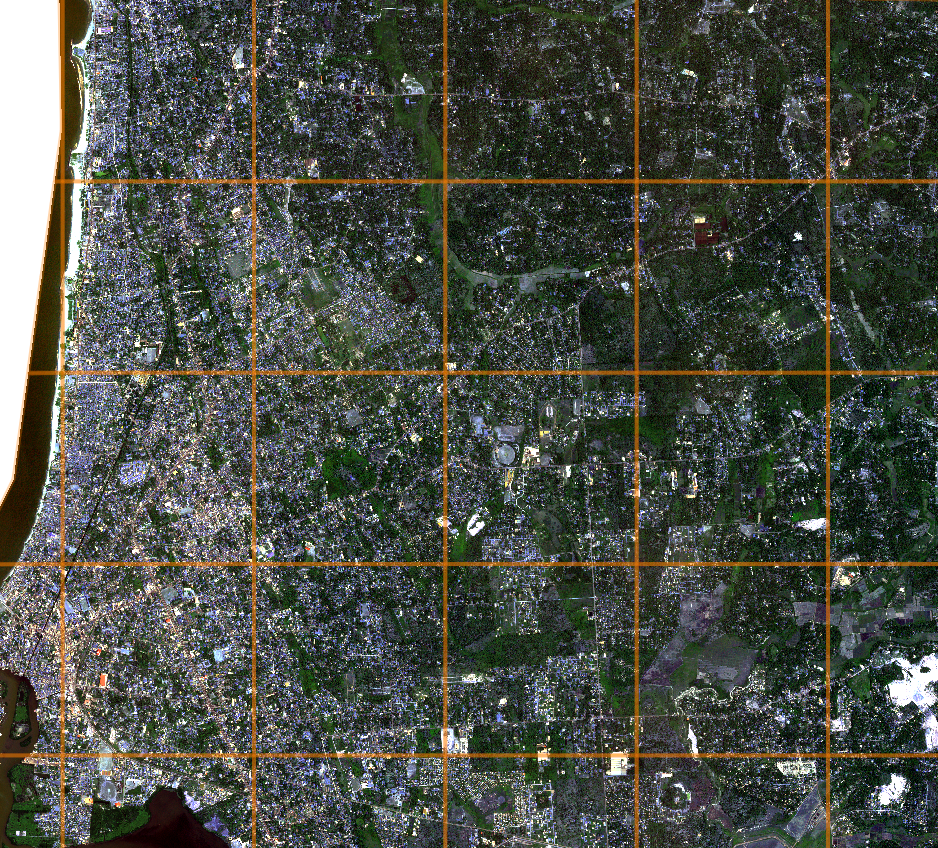
\includegraphics[width=0.9\textwidth]{images/negambo_with_clipped_grid_full.png}
    \caption[Creating a spatial grid] {Apply a spatial grid over each image,
      where the pixel size corresponds to an appropriate area for rescue
      decision-making.}
    \label{fig:biggrid}
  \end{figure}

This grid will be the basis for the aggregation of building counts. While in
practice the Bank or relief agency would assign the size of each grid
pixel--corresponding to the search and aid needs of a particular situation--for
the sake of a proof of concept the Datakind Team can assign a reasonably sized
grid at their convenience. A suitable size might have a grid square corresponds
to a square mile or square kilometer area. 

The grid can be converted to a shapefile and each grid pixel should be assigned as its own polygon and unique identification number. This step is critical because in the subsequent step, each grid pixel will be further broken down into a smaller grid of images. Unless the gridding is done correctly, there will be no way to reaggregate the building counts back to the larger spatial geometry. 

\subsection{Decompose each Grid Square into a Smaller Grid}

The original satellite images are too large to pass through the building
detector directly, hence these images must be cropped to a size that will
work best for the building detector, Figure \ref{fig:smallgrid}. The detector should work best when an
object within the image is between 40 to 400 pixels in size. This will rule out
very small objects whose features are difficult to identify, or very large
objects which are likely only partially captured in the image or represent
background noise. The original YOLO (You Only Look Once) object detector was trained for a size of
$419 \times 419$ pixels, though larger and smaller sized images have been used
before. Each square of the larger grid may correspond to a square mile or
square kilometer region, while each section of the smaller grid may correspond to a 100 or 200 meter square. 

\begin{figure}
	\centering
    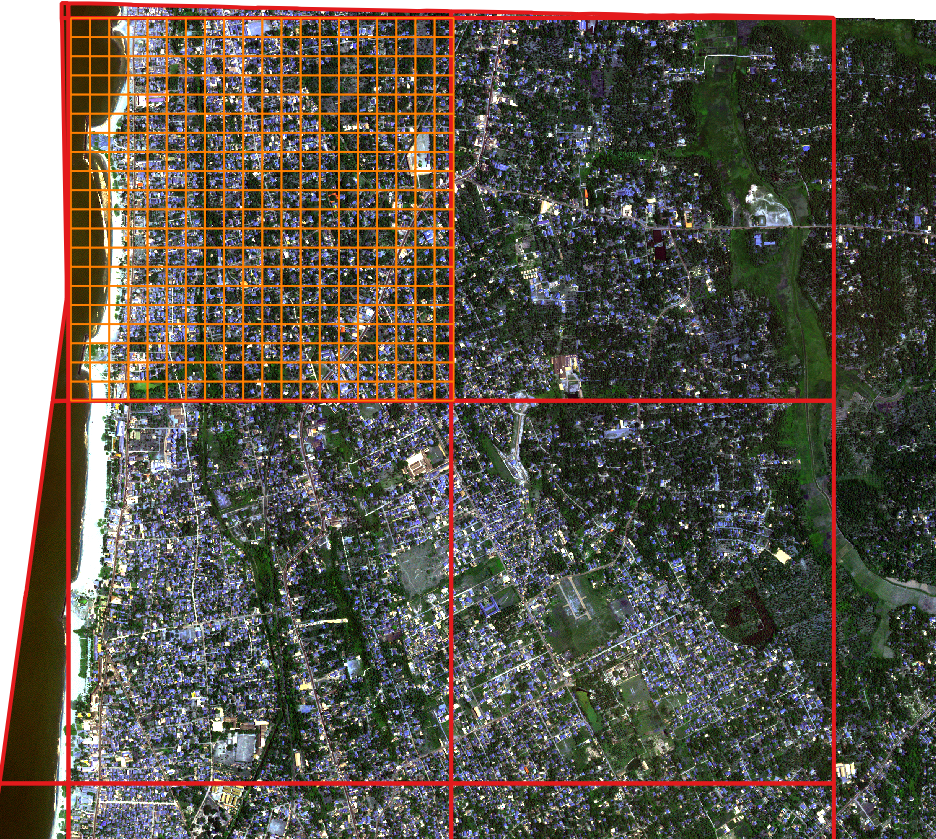
\includegraphics[width=0.9\textwidth]{images/negambo_subgrid_for_image_creation_transparent.png}
    \caption[Creating a spatial subgrid] {Apply a subgrid to the spatial grid to
    create smaller images that will fit within the specification of the object detector.}
    \label{fig:smallgrid}
  \end{figure}
  
Using the coordinates of each subgrid square, the original satellite image should be diced up into new smaller images corresponding to the smaller grid. These new images will be of a size suitable for building detection.

The name of each image should include the unique identifier of the larger grid square, as well as its own unique identifier. That way the building counts may be tallied by the larger grid locations. 

\subsection{Convert Smaller Images to 8 bit RGB PNG}

Convolutional Neural Networks generally work on PNG and JPEG image formats, while Satellite imagery is usually provided in GeoTiff format. The GeoTiff format is useful because it preserves the latitude and longitude information of each pixel, however this format is very memory intensive and can slow down model training and building detection.

The PNG and JPEG formats, while more compact, also strip all spatial coordinate information. Hence the coordinates in the PNG version of the image no longer reference latitude and longitude. Unless good metadata is maintained that links the PNG images back to the original images, the building detector will not be able to assign building counts back to the original map of the disaster affected area. 

\subsubsection{8 Bit RGB PNG Conversion}

The Python GDAL library, in particular the \mintinline{python}{Gdal_Translate}
function is useful in converting TIFF images to 8 bit PNG format. Most CNNs
require images to be in 8 bit format.

\subsubsection{Capture Metadata for Images}

Once the images are converted, the metadata for each image must be captured
in the metadata spreadsheet or dictionary.

\subsection{Label a Representative Sample of Images with Building Footprints}

Since the original building detector was trained on imagery from countries other than Sri Lanka, we should check to see just how accurately Sri Lanka buildings are detected. To execute this validation, the team can manually label a small number of the preprocessed images with building footprints. There are a variety of free softwares available to do this. 

The representative group may begin with about 50 images randomly selected from the set of pre-processed images. 

These 50 image and their labels are fed into the detector and then appropriate statistics are computed for accuracy, mAP, recall, etc. If the detection exceeds a certain threshold then the detector is labeled as valid. If there are substantial inaccuracies, then additional images may need to be labeled and additional training done on the model. 

To proceed, let us assume that the accuracy of building detection in the 50 images is acceptable.

\subsection{Predict Buildings in Representative Sample}

The next part of the process is to feed representative sample of images through
the building detector model. The model will predict the bounding box coordinates
and counts by image, Figure \ref{fig:predictions}. If the prediction accuracy on
the representative sample meets or exceeds 60 percent, then the team may
execute predictions on the entire set of pre-processed images. 

\begin{figure}
	\centering
    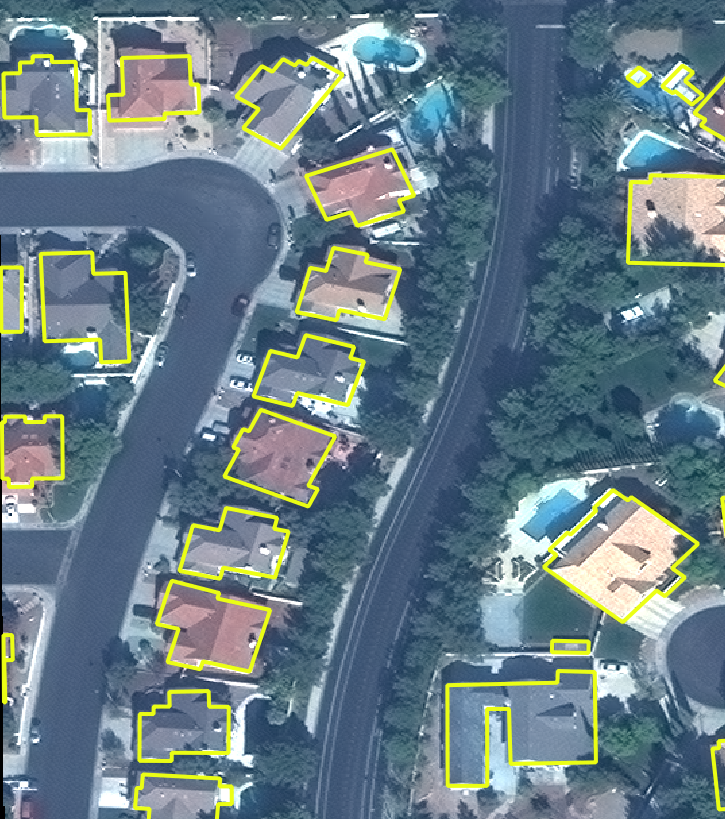
\includegraphics[width=0.7\textwidth]{images/detector_eg_edited.png}
    \caption[Building Footprint Prediction] {Predict building footprints for the
      representative sample of images.}
    \label{fig:predictions}
\end{figure}
\subsubsection{Aggregate all Building Counts by Grid Square}

Now that all of the buildings have been predicted, the building counts should be
aggregated by grid square. Since the names of each image should contain the
corresponding grid square, these counts should be easy to tally by grid square. 

\subsection{Formatting Data for Visualization}

Once the final tallies are computed, the results should be formatted into a spreadsheet or map to show the building counts by grid square.

\section{Conclusion}

This document identifies a step to generate building predictions from the raw
satellite imagery provided by the World Bank. While this is not the only
approach to solving this problem, it provides a benchmark or starting point for
any alternative approaches. 











%----------------------------------------------------------------------------------------
%	BIBLIOGRAPHY
%----------------------------------------------------------------------------------------

\renewcommand{\refname}{\spacedlowsmallcaps{References}} 

\bibliographystyle{unsrt}

\bibliography{review.bib}

%----------------------------------------------------------------------------------------

\end{document}
